% fluxograma.tex
\documentclass[border=10pt]{standalone}
\usepackage{tikz}
\usetikzlibrary{arrows.meta, positioning, shapes.geometric, calc}

\begin{document}
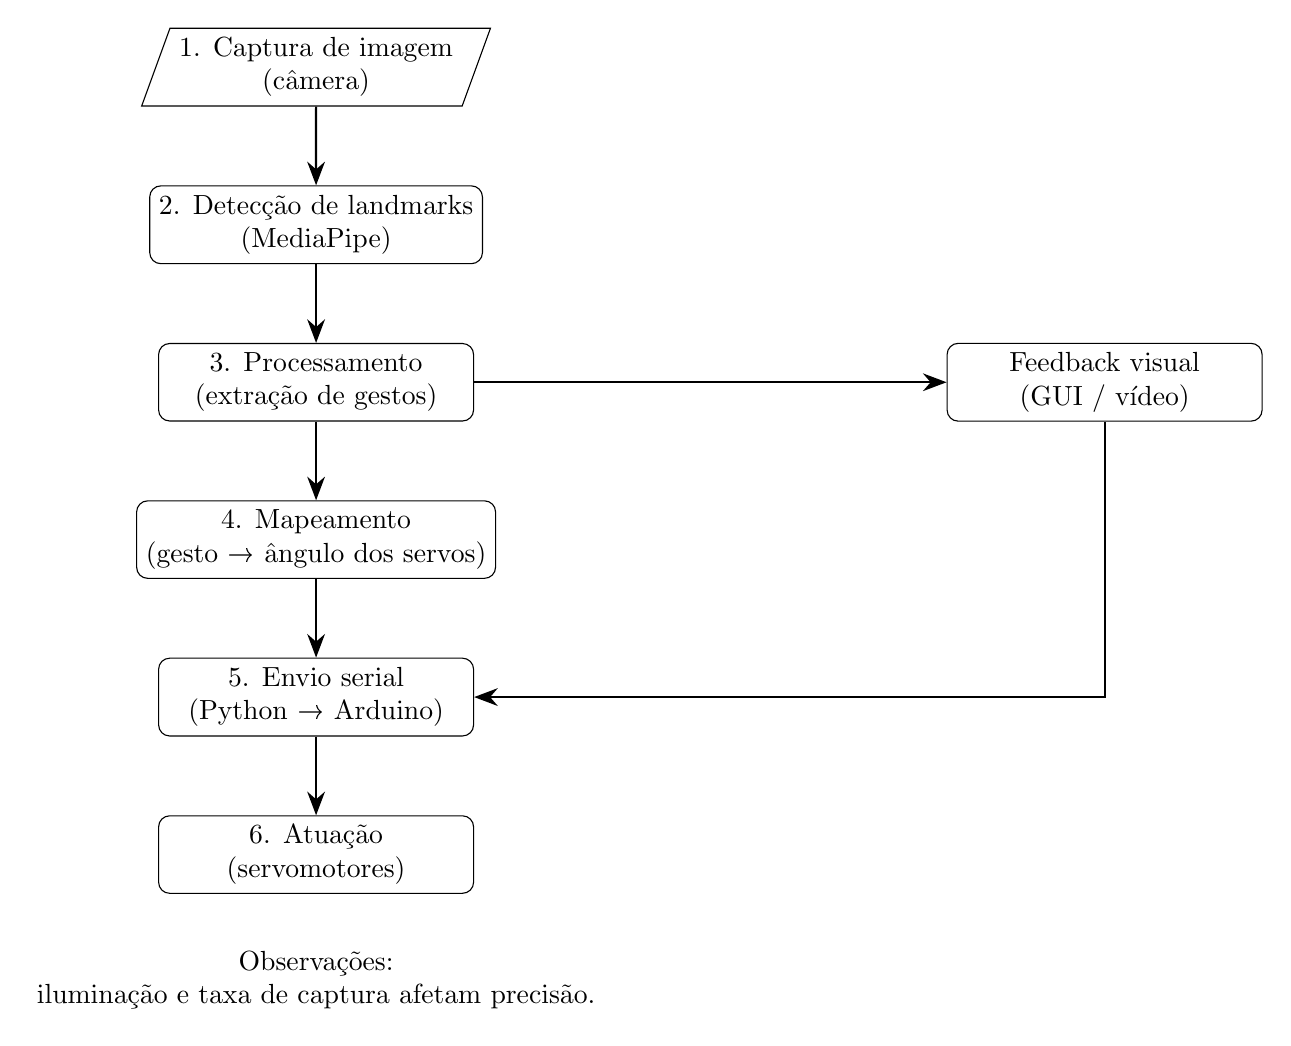
\begin{tikzpicture}[
  node distance=10mm and 25mm,
  box/.style={draw, rounded corners, minimum width=40mm, minimum height=8mm, align=center},
  io/.style={draw, trapezium, trapezium left angle=70, trapezium right angle=110, minimum width=40mm, minimum height=8mm, align=center},
  arrow/.style={-{Stealth[length=3mm]}, thick}
  ]

% Nodes
\node[io] (cam) {1. Captura de imagem\\(câmera)};
\node[box, below=of cam] (detect) {2. Detecção de landmarks\\(MediaPipe)};
\node[box, below=of detect] (process) {3. Processamento\\(extração de gestos)};
\node[box, below=of process] (map) {4. Mapeamento\\(gesto → ângulo dos servos)};
\node[box, below=of map] (send) {5. Envio serial\\(Python → Arduino)};
\node[box, below=of send] (act) {6. Atuação\\(servomotores)};
\node[box, right=of process, xshift=35mm] (visual) {Feedback visual\\(GUI / vídeo)};

% Arrows
\draw[arrow] (cam) -- (detect);
\draw[arrow] (detect) -- (process);
\draw[arrow] (process) -- (map);
\draw[arrow] (map) -- (send);
\draw[arrow] (send) -- (act);
\draw[arrow] (process) -- (visual);
\draw[arrow] (visual) |- (send);

% Optional annotations
\node[below=6mm of act, align=center] (note) {Observações:\\iluminação e taxa de captura afetam precisão.};

\end{tikzpicture}
\end{document}

